
%(BEGIN_QUESTION)
% Copyright 2013, Tony R. Kuphaldt, released under the Creative Commons Attribution License (v 1.0)
% This means you may do almost anything with this work of mine, so long as you give me proper credit

A {\it reciprocating} pump or compressor uses the back-and-forth motion of a piston within a cylinder to move fluid.  In the following example, the piston's reciprocating motion is controlled by a {\it crank} on a rotating shaft.  As the shaft turns, the crank causes the piston to move back and forth within the cylinder:

$$\includegraphics[width=15.5cm]{i02695x01.eps}$$

\underbar{file i02695}
%(END_QUESTION)





%(BEGIN_ANSWER)

 
%(END_ANSWER)





%(BEGIN_NOTES)


%INDEX% Machine, reciprocating compressor

%(END_NOTES)


